\documentclass[article,colorback,accentcolor=tud4c]{tudreport}
\usepackage[english]{babel}

\usepackage[stable]{footmisc}
\usepackage{hyperref}
\usepackage{color}

\usepackage{longtable}
\usepackage{multirow}
\usepackage{booktabs}
\usepackage{url}
\def\UrlBreaks{\do\A\do\B\do\C\do\D\do\E\do\F\do\G\do\H\do\I\do\J
	\do\K\do\L\do\M\do\N\do\O\do\P\do\Q\do\R\do\S\do\T\do\U\do\V
	\do\W\do\X\do\Y\do\Z\do\[\do\\\do\]\do\^\do\_\do\`\do\a\do\b
	\do\c\do\d\do\e\do\f\do\g\do\h\do\i\do\j\do\k\do\l\do\m\do\n
	\do\o\do\p\do\q\do\r\do\s\do\t\do\u\do\v\do\w\do\x\do\y\do\z
	\do\.\do\@\do\\\do\/\do\!\do\_\do\|\do\;\do\>\do\]\do\)\do\,
	\do\?\do\'\do+\do\=\do\#}

\usepackage{enumitem}
\setenumerate[1]{itemsep=0pt,partopsep=0pt,parsep=\parskip,topsep=5pt}
\setitemize[1]{itemsep=0pt,partopsep=0pt,parsep=\parskip,topsep=5pt}
\setdescription{itemsep=0pt,partopsep=0pt,parsep=\parskip,topsep=5pt}

\renewcommand {\thetable} {\arabic{section}.\arabic{table}}
\renewcommand {\thefigure} {\arabic{section}.\arabic{figure}}

\hypersetup{%
  pdftitle={TUD Corporate-Design f"ur {\LaTeX}},
  pdfauthor={C. v. Loewenich und J. Werner},
  pdfsubject={Beispieltext},
  pdfview=FitH,
  pdfstartview=FitV
}

\setcounter{seclinedepth}{1}

%%% Zum Tester der Marginalien %%%
  \newif\ifTUDmargin\TUDmarginfalse
  %%% Wird der Folgende Zeile einkommentiert,
  %%% werden Marginalien gesetzt.
  % \TUDmargintrue
  \ifTUDmargin\makeatletter
    \TUD@setmarginpar{2}
  \makeatother\fi
%%% ENDE: Zum Tester der Marginalien %%%

\newlength{\longtablewidth}
\setlength{\longtablewidth}{0.7\linewidth}
\addtolength{\longtablewidth}{-\marginparsep}
\addtolength{\longtablewidth}{-\marginparwidth}


% \settitlepicture{tudreport-pic}
% \printpicturesize

\title{Industrial Internship Report}
\subtitle{Letian Feng}
\subsubtitle{2255840\\
ETiT - Datentechnik\\
letian.feng@hotmail.com\\
31.12.2017
}
\setinstitutionlogo[width]{SAP_logo}

\begin{document}
\maketitle
\begin{abstract}

This report records my experience as a software developer intern in the team \textit{Big Data Vora} of the company SAP headquarters in Walldorf, Baden-W{\"u}rttemberg, Germany.

SAP(\textbf{S}ystems, \textbf{A}pplications \& \textbf{P}roducts in Data Processing), is the world leader in enterprise applications in terms of software and software-related service revenue. \cite{sap company information}
The team \textit{Big Data Vora} focuses on processing big data in distributed systems, especially on computing clouds like Amazon AWS and Microsoft Azure. 
Now this team is working on \href{https://www.sap.com/products/data-hub.html}{\textcolor{blue}{SAP Data Hub}}, which is a brand new data processing platform and the base of SAP's next generation products like Leonardo. 
In the end, SAP Data Hub should be able to run both SAP and non-SAP services, just like SAP's motto - Run Simple.

From my view as a developer, SAP Data Hub consists of 3 parts: 
\begin{itemize}\itemsep-\the\parsep
	\item SAP Vora, the infrastructure, distributed database system for big data processing. It contains a series of data processing engines, a transaction coordinator, and several interfaces to import data from different sources;
 	\item vFlow, backend service. It is a pipeline system helping customers to define their data flows running on SAP Vora or other data processing tools;
 	\item Web UI, frontend interface for the vFlow.
\end{itemize}

More detailed information about SAP Data Hub will be given in the following sections.

My work is almost all about an operator in the vFlow system - \textbf{Livy Spark Submit}. It submits data processing jobs to the Livy server in a remote cluster, it also retrieves the execution results or errors when the jobs succeed or fail.

In the past, only users, who have logged into a cluster, could submit data processing jobs to the cluster. If a user wants to submit another job to another cluster, then he has to log out and log in to the other cluster and finally submit it, obviously this is very inefficient. In addition, it could be very insecure as well, because those users are also allowed to see or even change system settings, which are not relevant to job submission, e.g. remove all system files. 

Therefore, we developed this Livy operator, with which users could submit their jobs remotely to multiple clusters without login, but only authenticated users' submissions will be accepted. This operator provides users the opportunity to scale out their computing capacity transparently, i.e. install more nodes in a cluster or deploy more clusters; on the other hand, it gives cluster administrators the ability to protect their computing nodes from unauthenticated users. In short, the Livy operator kills two birds with one stone.

Basically, my contribution could be split into 4 parts: 

\begin{itemize}\itemsep-\the\parsep
	\item Proof of Concept;
	\item Source Code Implementation;
	\item Error Handling and Monitoring Improvement;
	\item Unit Tests \& Docker-based Integration Tests;
\end{itemize}

To accomplish the above tasks, following technologies and programming languages were used: 

\begin{itemize}\itemsep-\the\parsep
	\item 
	\href{http://hadoop.apache.org/}{\textcolor{blue}{Hadoop}}, \href{https://spark.apache.org/}{\textcolor{blue}{Spark}},
	\href{https://en.wikipedia.org/wiki/Linux}{\textcolor{blue}{Linux}}, \href{https://www.docker.com}{\textcolor{blue}{Docker}}, \href{https://livy.incubator.apache.org/}{\textcolor{blue}{Livy}}, \href{https://www.sap.com/products/hana-vora-hadoop.html}{\textcolor{blue}{SAP Vora}}, \href{https://web.mit.edu/kerberos/}{\textcolor{blue}{Kerberos}}, \href{https://git-scm.com/}{\textcolor{blue}{Git}}, \href{https://en.wikipedia.org/wiki/Markdown#Implementations}{\textcolor{blue}{Markdown}},
	\href{https://www.wireshark.org/}{\textcolor{blue}{Wireshark}} \& \href{https://kubernetes.io/}{\textcolor{blue}{Kubernetes}};
	\item 
	\href{https://golang.org/}{\textcolor{blue}{Go}}, \href{https://www.gnu.org/software/bash/}{\textcolor{blue}{Bash}} \& \href{https://www.scala-lang.org/}{\textcolor{blue}{Scala}}. 
\end{itemize}

The report introduces a lot of technical details, encountered challenges and even some bugs. Features will be illustrated by pictures, but no source code will be shown due to confidential reasons. All code were pushed into SAP's internal GitHub.
\end{abstract} 
\newpage

\tableofcontents
%\part{Lorem Ipsum (\textbackslash part)\label{part_lorem}}
\newpage

\section{Introduction}
\setcounter{table}{0}
\setcounter{figure}{0}

SAP Data Hub is a DataOps management solution that enables agile data operations across the enterprise. It supports data sharing, pipelining, and governance of all data in the connected landscape.\cite{sap data hub}

The SAP Data Hub product is composed of several components\cite{data hub architecture}:
\begin{itemize}\itemsep-\the\parsep
\item An application tier (control plane) based on SAP HANA extended application services (XS), advanced model.
\item The core distributed runtime (based on SAP Vora) installed on a Kubernetes cluster.
\item Extensions to the Spark environment on a Hadoop cluster.
\item The SAP Data Hub adapter agent installed on one edge node of the Hadoop environment.
\end{itemize}

Figure 1.1 outlines the deployment view of SAP Data Hub.

\begin{figure}[!h]
   	\centering
   	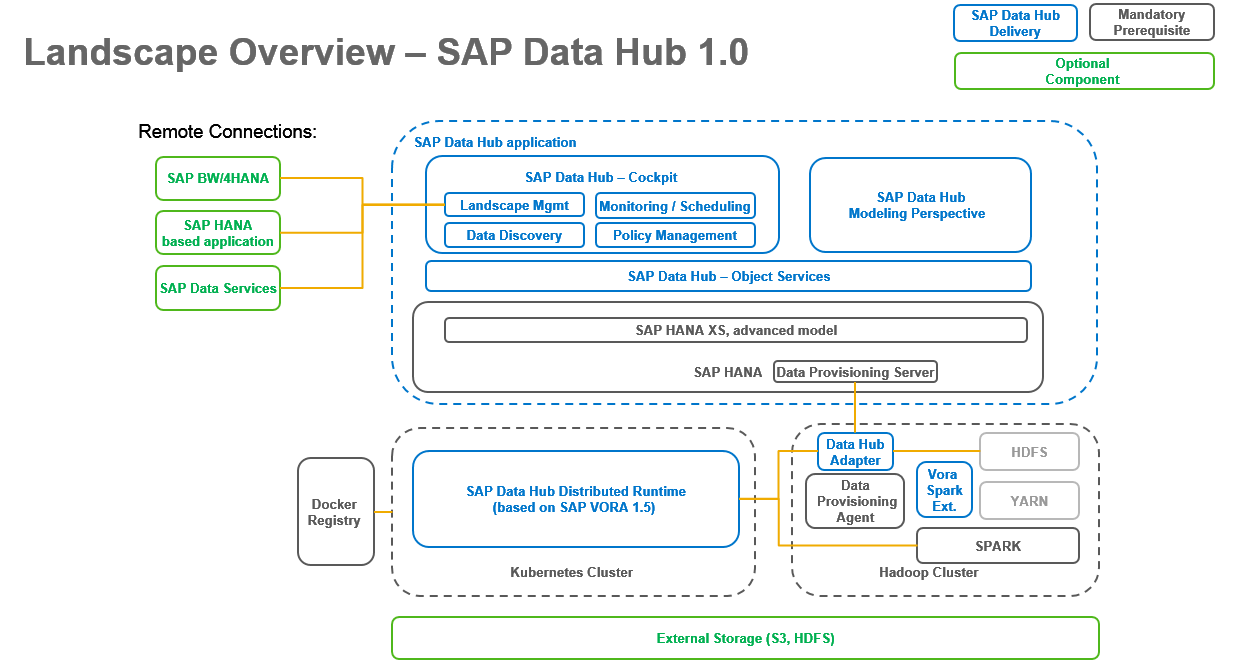
\includegraphics[width=\textwidth]{architecture}
   	\caption{Architecture of SAP Data Hub\cite{data hub architecture}}
\end{figure}

All data services are running in the top level - the application tier. With Data Hub Cockpit, data services can generate data processing pipelines, each pipeline contains a series of operations, e.g. load data from a file in HDFS, filter something, and then output in the web page. Sometimes users want to DIY their own data processing pipelines, then they can use Data Hub Modeling Perspective, which is actually the web UI of vFlow mentioned in the abstract. Pipelines will be passed from Data Provisioning Server to Data Hub Adapter. 

Data Hub Adapter is the central communication endpoint for operations performed from SAP Data Hub application on SAP Data Hub Distributed Runtime(SAP Vora, vFlow, and Hadoop). With help of Data Hub Adapter, pipelines will be sent to the Distributed Runtime and be executed there.

\begin{figure}[!h]
	\centering
	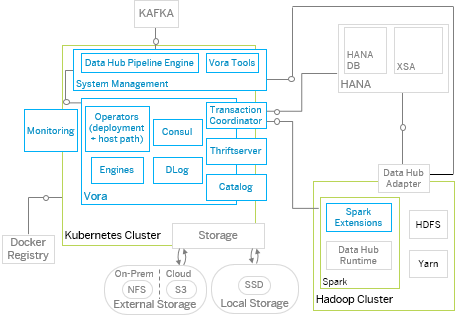
\includegraphics{vora}
	\caption{A high-level overview of the SAP Data Hub Distributed Runtime\cite{vora and data hub}}
\end{figure}

As shown in the figure 1.2, we can know more about SAP Data Hub Distributed Runtime and how a pipeline is executed. First, the Data Hub Adapter gives the pipeline received from the application tier to Data Hub Pipeline Engine in the Kubernetes cluster. If the pipeline contains a Spark/Vora job, this job will be sent back to Data Hub Adapter, then a Spark client will submit the job to the scheduler YARN. YARN will allocate computing resources for it. If it's only a simple Spark job, it runs only in the Hadoop cluster; but if it's also a Vora job, an external library "Vora Spark Extension" will be invoked to submit queries to Vora Transaction Coordinator(TC) in the Kubernetes cluster. TC controls the execution of queries on several engines for different functions - relational, graph, time series and document engine. After all queries are executed, results will be returned, Spark jobs and the pipeline will be finished step by step, final results will be displayed on the web UI. 

However, in this report, we don't need to discuss all details of SAP Data Hub. Figure 1.3, which only shows the interfaces of SAP Data Hub, is a easier way to understand it:

\begin{figure}[!h]
	\centering
	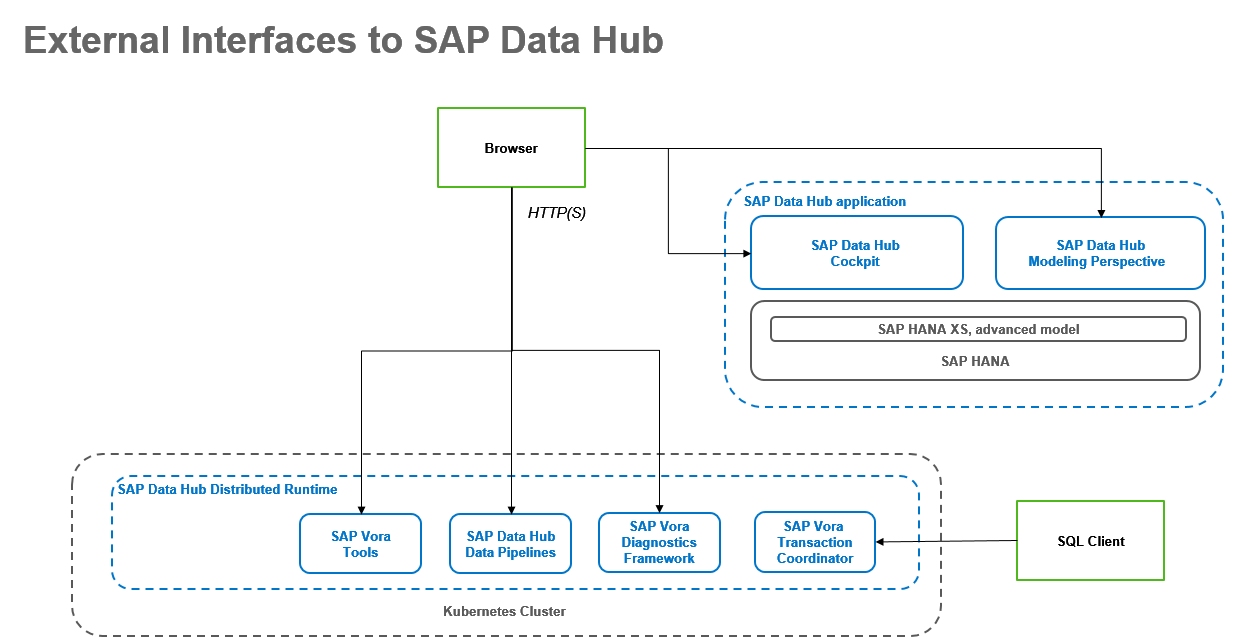
\includegraphics[width=\textwidth]{interfaces}
	\caption{Interfaces of SAP Data Hub\cite{data hub architecture}}
\end{figure}

Users always use their web page browser to access SAP Data Hub. They use either a data service in SAP Data Hub Cockpit to generate a data processing pipeline, or use SAP Data Hub Modeling Perspective to DIY a pipeline. The pipeline will be given to a SQL client, and this SQL client will communicate with the Transaction Coordinator in SAP Data Hub Distributed Runtime, so that data could be processed correctly. During the execution users should also be able to monitor pipeline's status via Diagnose Framework, and they can check the final results with Vora Tools after the pipeline is finished. Both Diagnose Framework and Vora Tools are accessible in the browser.

\newpage

\section{Proof of Concept}
\setcounter{table}{0}
\setcounter{figure}{0}

SAP Data Hub version 1.0 was released in September 2017, and then version 1.2 was released in December 2017. As the core component of the Data Hub Distributed Runtime, SAP Vora also keeps evolving itself. When I started my internship, Vora released v1.4, then in September Vora v2.0 was released, and in December was Vora v2.1. Their architectures are shown in the following pictures:

In Vora v1.4, there were many components, their relationships and dependencies were very complex, both Vora engines and Spark nodes are running on the same cluster.

\begin{figure}[!h]
	\centering
	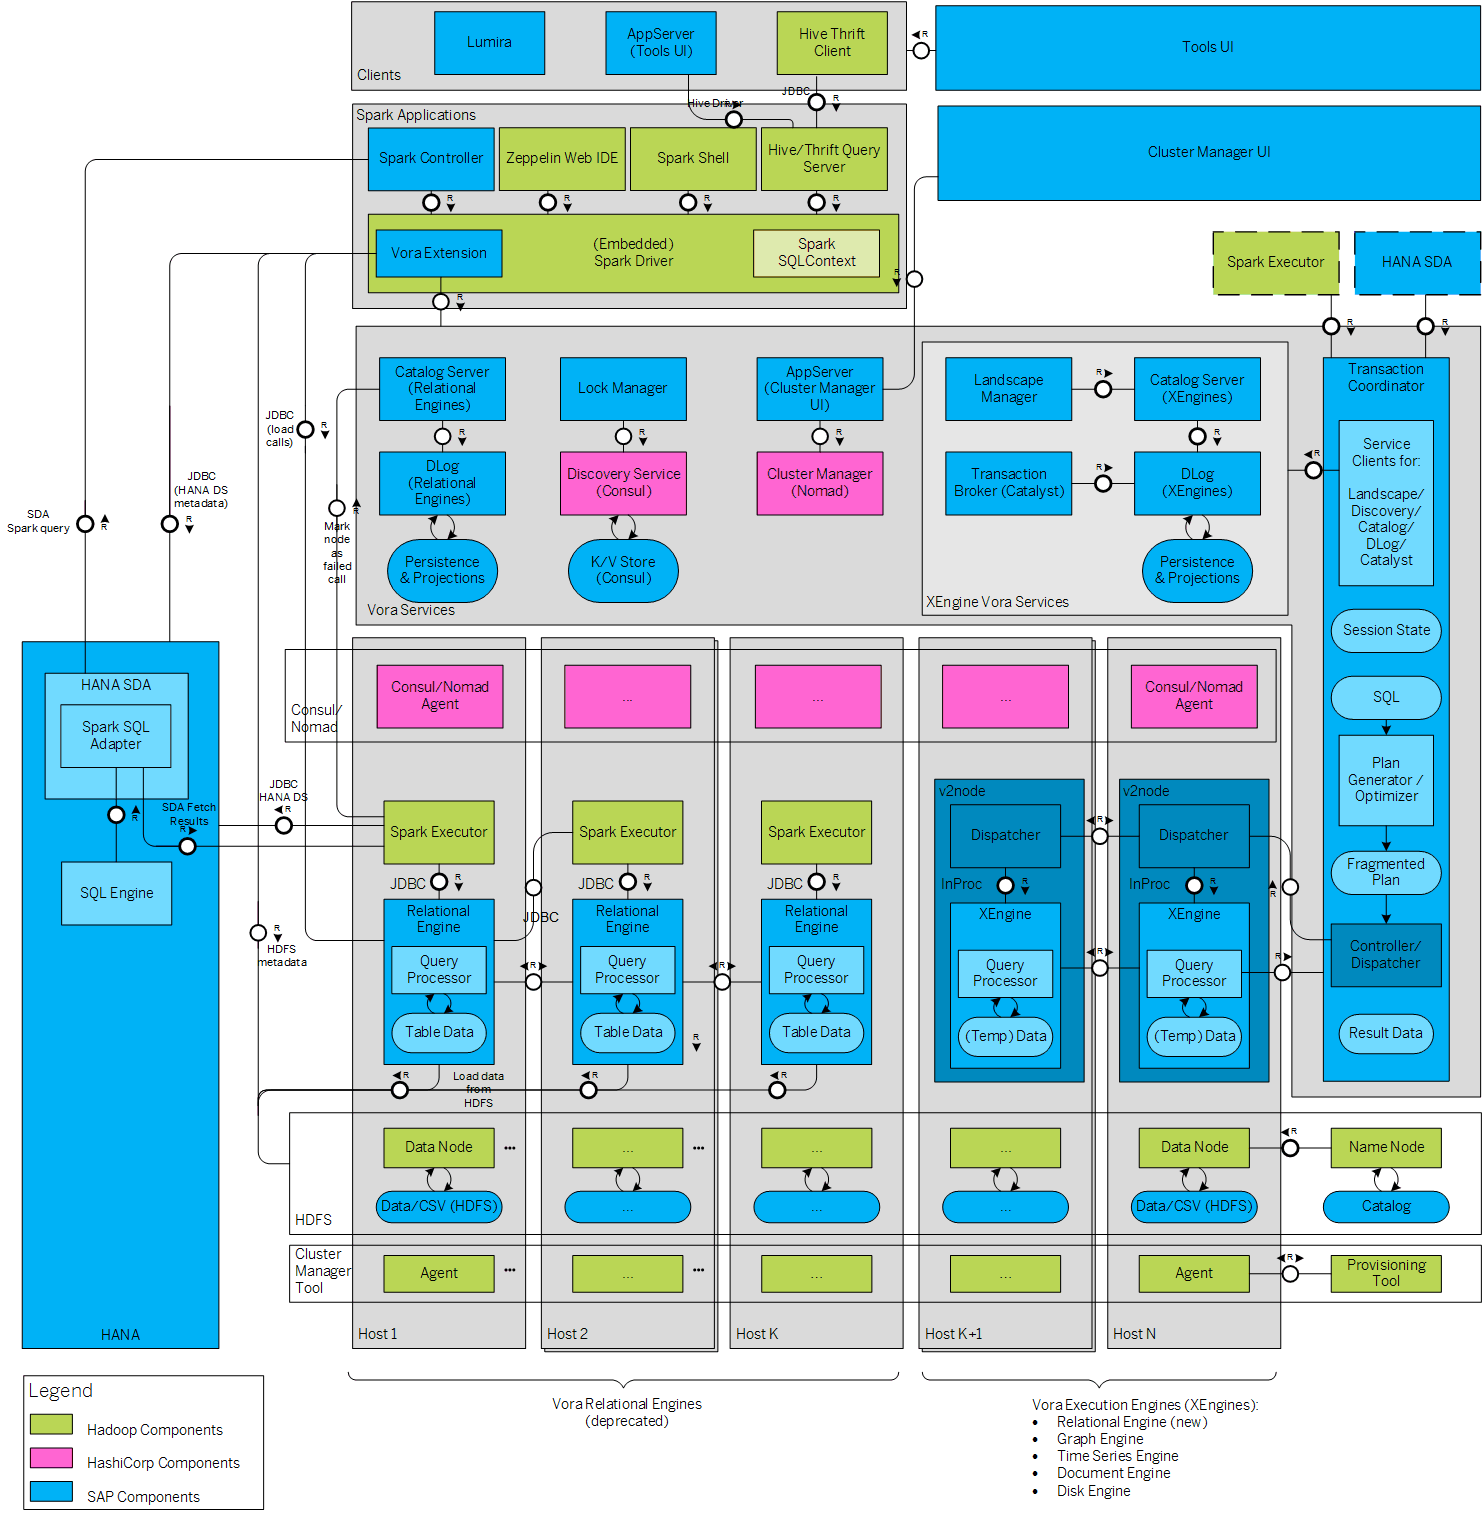
\includegraphics[width=0.9\textwidth]{vora14}
	\caption{SAP Vora Architecture version 1.4\cite{vora 1.4 architecture}}
\end{figure}

In Vora v2.0, all Vora components were encapsulated in Docker\footnote{Docker is a tool that can package an application and its dependencies in a virtual container that can run on any Linux server. This helps enable flexibility and portability on where the application can run, whether on premises, public cloud, private cloud, bare metal, etc.} containers and managed by a Kubernetes\footnote{Kubernetes is an open-source platform designed to automate deploying, scaling, and operating application containers. It supports a range of container tools, including Docker.} cluster, only few things like Spark workers and the Vora Spark Extension remain in the original Hadoop cluster. In this way, all Vora services are separated from the computing resources in the Hadoop cluster. With help of Kubernetes, all Vora services could be easily deployed and seamlessly updated or reverted.

\begin{figure}[!h]
	\centering
	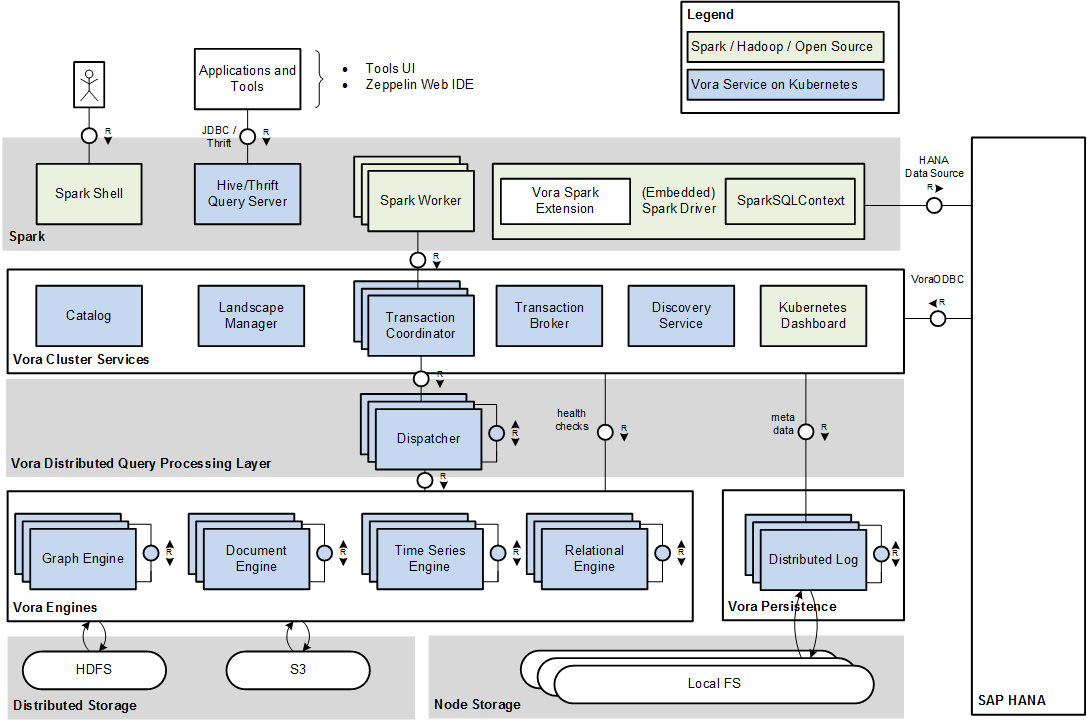
\includegraphics[width=0.9\textwidth]{vora20}
	\caption{SAP Vora Architecture version 2.0\cite{vora 2.0 architecture}}
\end{figure}

Finally, in Vora v2.1, Livy shows up for the first time, and it becomes the most preferred Spark client in the Hadoop cluster to submit Spark/Vora jobs.

\begin{figure}[!h]
	\centering
	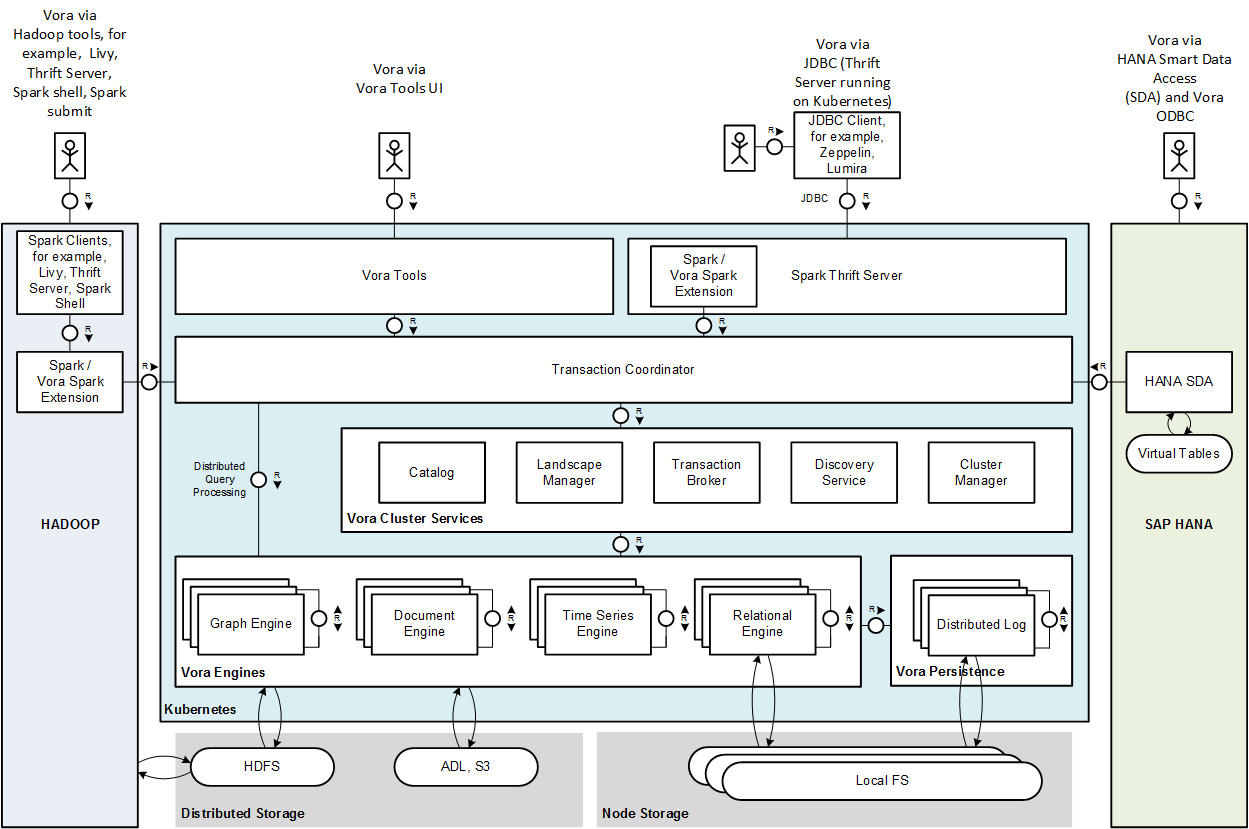
\includegraphics[width=0.9\textwidth]{vora21}
	\caption{SAP Vora Architecture version 2.1\cite{vora 2.1 architecture}}
\end{figure}

The 2 changes in v2.0 and v2.1 have very important effects:

\begin{enumerate}
	\item Separate Vora from the Hadoop cluster, put it in a Kubernetes cluster:
	\begin{itemize}
		\item Lower system coupling, higher computing efficiency;
		\item Easier to manage and secure Vora components;
		\item Kubernetes makes it possible to update or revert Vora version seamlessly.
	\end{itemize}
	\item Add a Spark client Livy in the Hadoop cluster:
	\begin{itemize}
		\item Possible to submit jobs to a remote Hadoop cluster;
		\item Possible to submit jobs with username, only authenticated users' requests could be passed, higher security;
		\item A Vora cluster could access multiple Hadoop clusters, scale out computing resources, not scale up.
	\end{itemize}
\end{enumerate}

Since those 2 changes mean a lot, they must be proved before being implemented - Proof of Concept, as known as POC. I was responsible to  the POC of Livy, it consists of 4 steps, I will describe them in the following 4 subsections.

	\subsection{Prove that Livy could submit Spark jobs to a simple cluster}
	Actually, Spark job submission is exactly Livy's function\footnote{Livy's official definition: \textit{Apache Livy is a service that enables easy interaction with a Spark cluster over a REST interface. \textbf{It enables easy submission of Spark jobs or snippets of Spark code}, synchronous or asynchronous result retrieval, as well as Spark Context management, all via a simple REST interface or an RPC client library.\cite{what is livy}}}. However, a software engineer should never simply believe in documentations, there are usually hundreds of bugs in every software. Therefore, experiments are always required before a technology is used in the production environment.
	
	Before we start to prove, let me explain what is a Spark job and how it is submitted in the traditional way. A job is actually an application that running on a cluster. Once an user application is bundled, it can be launched using the spark-submit\footnote{The spark-submit script in Spark's bin directory is used to launch applications on a cluster. It can use all of Spark’s supported cluster managers through a uniform interface.\cite{spark submit}} script. This script takes care of setting up the classpath with Spark and its dependencies, and can support different cluster managers and deploy modes that Spark supports. The format of executing spark-submit is:
	
	\noindent\textbf{spark-submit --class <main-class> --master <master-url> ... <application-jar> [application-arguments]}
	
	Obviously, to submit a job, we need at least a class name, a path to the application JAR\footnote{A JAR (Java ARchive) is a package file format typically used to aggregate many Java class files and associated metadata and resources (text, images, etc.) into one file for distribution.\cite{jar}}, a cluster manager. For example, the following command runs a Pi-calculating-job saved in the default Spark examples JAR on a cluster managed by YARN\footnote{Hadoop YARN, a platform responsible for managing computing resources in clusters and using them for scheduling users' applications.\cite{hadoop}}, the JAR file is stored in HDFS\footnote{Hadoop Distributed File System(HDFS), a distributed file-system that stores data on commodity machines, providing very high aggregate bandwidth across the cluster.\cite{hadoop}} and this job will be split into 10 partitions:
	
	\noindent\textbf{spark-submit --class org.apache.spark.examples.SparkPi   --master yarn-cluster hdfs:///tmp/spark-examples.jar 10}
		
	Now let's see how can we submit a Spark job through Livy. First, we need to install Livy on our cluster and run Livy's RESTful service\footnote{Representational state transfer (REST) or RESTful web services are a way of providing interoperability between computer systems on the Internet. REST-compliant Web services allow requesting systems to access and manipulate textual representations of Web resources using a uniform and predefined set of stateless operations.\cite{rest}}. According to \href{https://livy.incubator.apache.org/docs/latest/rest-api.html}{\textcolor{blue}{Livy's REST API}}, we can send POST/GET/DELETE requests to the Livy server to submit, monitor, and cancel Spark jobs. To submit a job, we need to send a POST request with data options like "file", "className", and "args" to the URI(Uniform Resource Identifier) /batches. 
	
	In command line mode, we usually use the tool curl\footnote{cURL is a computer software project providing a library and command-line tool for transferring data using various protocols.\cite{curl}} to send requests, for example, the following command sends a job submission request which is identical as the spark-submit request above:
	
	\noindent\textbf{curl -v \$LIVY\_URL/batches -X POST -H "Content-Type:application/json" --data '\{"file":"/tmp/spark-examples.jar", "className":"org.apache.spark.examples.SparkPi", "args":["10"]\}'}
	
	After sending this POST request to Livy and checking the cluster manager YARN's UI, we could find that a job "org.apache.spark.examples.SparkPi" is accepted and finished with a result like "Pi is roughly 3.13918". So it is proved that Livy could submit Spark jobs to a simple cluster.
		
	\subsection{Prove that Livy could submit Vora jobs to a simple cluster}
	
	First of all, I deployed a Vora cluster without Kerberos and installed Livy, then started services HDFS, YARN, Livy, and Vora Tools. After uploaded the Vora Spark Extension "spark-sap-datasources.jar" to the HDFS, I sent the Vora job submission request to Livy:
	
	\noindent\textbf{curl -v \$LIVY\_URL/batches -X POST -H "Content-Type:application/json" -H "X-Requested-By: hdfs" --data '\{"file": "/tmp/spark-sap-datasources.jar", "className":"com.sap.spark.vora.examples.LoadDataIntoVora","args":["10"]\}'}
	
	Because the Vora cluster enables the CSRF protection\footnote{Cross-site request forgery is a type of malicious exploit of a website where unauthorized commands are transmitted from a user that the web application trusts.\cite{csrf}} by default, this request has an additional header "X-Requested-By: hdfs". The application jar is not spark-examples.jar any more, but our Vora Spark Extension. This job does nothing but load data from some csv-files saved in HDFS to Vora. As same as in the subsection 2.1, this job could always be accepted and executed by YARN. If we check the Vora Tools we started at the beginning, we can find that data is already loaded into Vora. So it is proved that Livy could submit Vora jobs to a simple cluster.
		
	\subsection{Prove that Livy could submit Spark jobs to a Kerberized cluster}
	
	In the last 2 subsections, we have proved that Livy fulfills our expectation for remote submission. However, Livy has a feature - impersonation. It provides users the possibility to submit jobs as other users and even administrator, this could lead to security problem, so Kerberos is introduced to secure the Vora cluster.
	
	Kerberos is a computer network authentication protocol that works on the basis of tickets to allow nodes communicating over a non-secure network to prove their identity to one another in a secure manner. Its designers aimed it primarily at a client-server model and it provides mutual authentication-both the user and the server verify each other's identity. Kerberos protocol messages are protected against eavesdropping and replay attacks.\cite{kerberos} More detailed description about the protocol please see in this \href{https://en.wikipedia.org/wiki/Kerberos_(protocol)#Description}{\textcolor{blue}{link}}.
	
	\begin{figure}[!h]
		\centering
		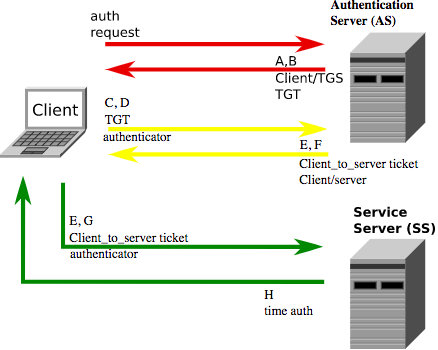
\includegraphics[width=0.5\textwidth]{Kerberos}
		\caption{Kerberos Authentication Procedure\cite{kerberos}}
	\end{figure}
	
	Specifically, we need to deploy clusters secured by Kerberos, and then create a Kerberos principal with our username \& password in the Authentication Server(AS), and generate a encrypted keytab(key table) based on this principal. Since then, all authentications will be done based on this keytab, so that the password will not be exposed during transfer in networks. After that, we copy the encrypted keytab to our client machine and set its \href{https://en.wikipedia.org/wiki/File_system_permissions#Numeric_notation}{\textcolor{blue}{file permission}} as "-rwx------", which means read, write, \& execute only for owner. This ensures that other users are not allowed to access the keytab, so they have no chance to get authenticated as us. In the end, we execute the following command on the client machine to get authenticated and we can use all services like before, e.g. Livy, HDFS, Vora, etc.
	
	\noindent\textbf{kinit -k -t /etc/security/keytabs/livy.service.keytab username/realmname}
	
	After running this command, we are authenticated and have a ticket granting ticket(TGT), now we are allowed to send job submission requests. In addition, since we are authenticated, we cannot use Livy's impersonation feature anymore, so our security requirement is fulfilled.
	
	The command for secure job submission is a little bit different from the one in subsection 2.1:
	
	\noindent\textbf{curl -v --negotiate -u : \$LIVY\_URL/batches -X POST -H "Content-Type:application/json" -H "X-Requested-By: hdfs" --data '\{"file":"/tmp/spark-examples.jar","className":"org.apache.spark.examples.SparkPi","args":["10"]\}'}
	
	With the option "--negotiate -u :", curl is able to request client to server ticket from the AS, and then use this ticket to get Livy service from its Service Server(SS).
	
	Exactly same as the subsection 2.1, the job submission could be accepted and executed successfully. So it is proved that Livy could submit Spark jobs to a Kerberized cluster.
		
	\subsection{Prove that Livy could submit Vora jobs to a Kerberized cluster}
	
	At first, I thought that there is no difference between submitting a Vora job and a Spark job, but I was wrong - Kerberos protects not only the services Livy and Spark, but also Vora. Since Vora was still in development, there were 2 restrictions:
	
	\begin{enumerate}
		\item Almost all Kerberos configurations are hard-coded in the Vora and Spark config files, so changing Vora's Kerberos configurations is not supported;
		\item When Vora runs behind the Kerberos protection, it could be accessed only by the user vora, so in principle all the other users are not allowed to submit Vora jobs any more.
	\end{enumerate}
	
	This is a hard situation, that we cannot submit jobs as ourselves and we cannot change configurations to make it possible. In addition, as discussed in the chapter 2.3, theoretically once we are authenticated, we are not allowed to impersonate as another user such as the user vora.
	
	This difficulty made my work in a dilemma, I had proved everything but the most important part. After wasting almost 1 month for communicating with the security team in Turkey, and reading all kinds of documentations about Vora, Livy, and Kerberos, finally I found a very tricky solution - put users, which are allowed to use Vora, into Livy's superuser list. This makes it possible to let users get authenticated as themselves, and allow them to impersonate as the user vora so that they can submit Vora jobs as well.
	
	After submitting jobs and checking results as in the chapter 2.2, data is loaded into Vora, so it is proved that Livy could submit Vora jobs to a Kerberized cluster.\\
	
	Till now, the POC part is finally finished. The things I showed here is only a smart part of all I experienced, there were so many experiments and failures, but I can't write them all due to limited length. Anyway, I learned a lot during that time, the most important 2 things are:
	
	\begin{enumerate}
		\item Never simply believe in documentations, do experiments by yourself;
		\item Engineering is not perfectionism, tricky solutions are also solutions.
	\end{enumerate}
	
\newpage

\section{Source Code Implementation}
\setcounter{table}{0}
\setcounter{figure}{0}

After the POC of Livy was finished, I started to implement an Operator "Livy Spark Submit" in SAP Data Hub, specifically in vFlow. With this operator, a pipeline could submit Spark/Vora jobs directly to any remote Hadoop cluster, no matter it's Kerberized or not. 

	\subsection{Requirements}
	In software engineering, code implementation is not the most difficult part, but understanding requirements. If the product cannot fulfill users' expectation, then it makes no sense no matter how many lines of code are written and how beautiful is the coding style. 
	
	However, requirements could change over time. Sometimes only after a requirement is implemented, people can find out it is useful, or useless, maybe even wrong. Therefore, it's very important to keep communicating with people playing different roles. Although I am the only person writing code for this operator, there was always a weekly meeting, in which I, my tutor, the team leader, a security expert in Turkey and 3 technical consultants in the USA, shared the current development process, bugs, additional requirements and our opinions to the vision of this operator. Due to the length limit, I can't show all details in the meetings, let's simply see the final requirements for the operator "Livy Spark Submit":
	
	\begin{itemize}
		\item it works in SAP Data Hub Pipeline Modeler(vFlow);
		\item it could submit jobs to any remote cluster with Livy server;
		\item it could submit jobs to both simple and Kerberized clusters;
		\item it supports impersonation;
		\item it supports changing the name and configuration of jobs;
		\item it supports 2 error handling mode "default" and "pipeline". In the first mode, the pipeline fails when the operator fails. In the second mode, the operator's failure doesn't lead to pipelines failure, the operator outputs the error information via its output channel "outError";
		\item it supports 2 submission modes "jar" and "snippet". In the first mode it submits an job(application). In the second mode it maintains a session and sends several lines of spark code;
		\item for the "jar" mode, it specifies the path to the application jar, the class name and the arguments for execution;
		\item for the "snippet" mode, it specifies the code snippet and its language, and if the snippet is executed in the strict mode(the session stops when one line of code fails);
		\item it has 1 input channel. If no channel is set, it submits only once, when the whole pipeline is started. In the second way, it submits a job when an input signal arrives, no times limit;
		\item it has 2 output channels "outSuccess" and "outError" for outputting information when a job succeeds or fails.
	\end{itemize}
	
	\subsection{Implementation}
	
	Although there are so many requirements, actually the role of this operator is not so complex. It reads some configurations from the web UI, and then it sends requests to the Livy Server and retrieves status regularly, and in the end it posts success or failure information back to the web UI.
	
	As mentioned before, Livy provides a REST API for submitting jobs and retrieving job states and results. REST is an architecture style and it has 6 constraints(Server-Client mode, Stateless, Uniform Interface, Cache and Code-on-demand). In our case, we just need to know that Livy works in the Server-Client mode, the Livy server provides an uniform interface, so that a client could send requests according to the standard HTTP methods(e.g. GET, POST, DELETE) and the media type \textbf{application/json}, if everything runs properly, the client will get a HTTP response in the JSON format as well.
	
	In short, we need to implement a HTTP client plus some special logics to fulfill the above requirements. 
	
	Figure 3.1 shows a sketchy flowchart for the Livy operator. First of all, the operator creates an object/instance in the backend and starts its constructor. The constructor reads configurations from the web UI(frontend) and binds them to the object's attributes, then input and output channels and a new initialized HTTP(S) client will also be bound to the object's attributes. If a security context is mentioned in the configuration, the operator must get authenticated before doing other things. Then the HTTP(s) client checks whether the Livy Server, which is described by a URL in configurations, works properly. After that, the operator submits a jar job or a sequence of code snippets according to the configurations, and keeps checking the job state from the Livy server until the job is finished. Depending on the job succeeds or fails, the operator retrieves the result and posts it on the web UI, or retrieves error information(stack trace, job link, etc.) and handles it according to the error handling mode.
	
	Since the part of sending requests is used for several times, so it is described in detail on the right side of the picture. First, we need to construct the request body according to the JSON format. Second, add header(s), e.g. \textbf{Content-Type:application/json} for specifying the content type as JSON, \textbf{X-Requested-By: hdfs} for passing the CSRF protection. Then the URL and the method of the request should be specified so that it could be directed to the correct destination and be executed in the right way. After the request is accepted, in principle a response will come back, it will be unmarshalled to an object with expected class/type, and at last the required information should be extracted from the object properly.
	
	\begin{figure}[!h]
		\centering
		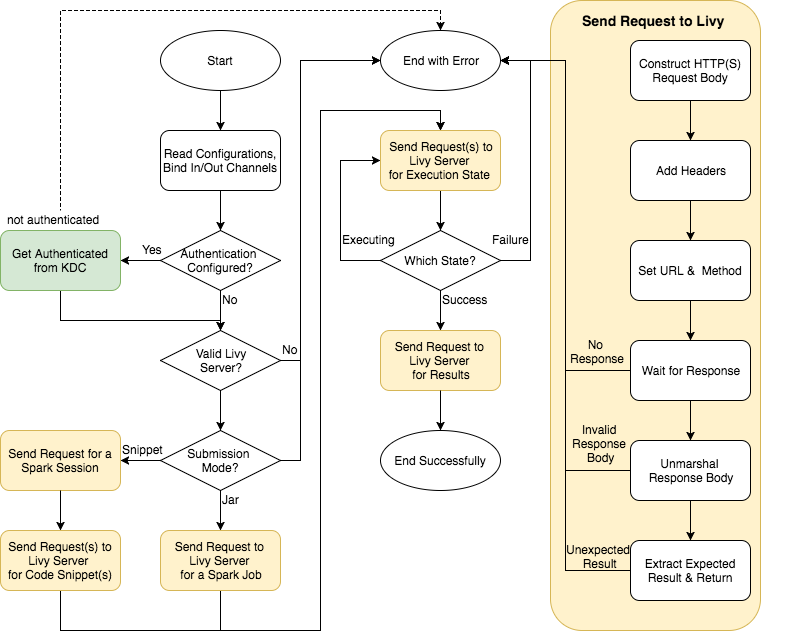
\includegraphics[width=0.8\textwidth]{flowchart}
		\caption{Basic Flowchart of Livy Spark Submit}
	\end{figure}
	
	\subsection{Code review and refactoring}
	
	Sometimes software could be written by only few people, even just one person alone. However, when a software has a large and complex architect, developers have to cooperate with each other to achieve releases before their deadlines. As the base of SAP's next generation products, SAP Data Hub is large and complex enough, so there are hundreds of developers working on it with full time. Unfortunately, not everyone is experienced, junior developers and interns like me usually write unscalable programs in ugly coding style with many bugs. Therefore, my code changes were always reviewed by some senior developers before the update was merged into the new version of SAP Data Hub.
	
	Thanks to the tool Git and the website GitHub, code review is much more easier than before. What I need to do is just commit my changes, and push those commits to a code repository on the SAP's internal GitHub, then a senior developer could see the difference between my version and the old one.
	
	If the reviewer thinks those updates are ok, then they will be merged into the master branch of the project and be part of the next possible release, otherwise the reviewer annotates at the problematic lines with their opinions and the changes will not be merged. In the second case, the reviewer will probably ask the person who submits those code to do a code refactoring - correct the code and make new commits again.
	
	During the internship I experienced several times of code review, sometimes I passed without any annotations, sometimes I had to change my implementation again and again. The most impressed one was in September, the reviewer thought my code was too messy and not scalable at all, he made more than 30 annotations and asked for a refactoring. I was really angry and ashamed, but I knew he was right. So I redesigned the flowchart, extracted some common code blocks to helping functions, generalized existing functions so that new features could be easily integrated, etc. After 2 weeks and more than 10 times communication, the new version was finally accepted and merged, both the reviewer and I were very happy, because we shortened the program from 1100 lines to only 800, the code style was much prettier than before, and the most important thing is that adding a new feature costs much less time than before - from 2-3 days to just 2 hours!
	
	Thanks to the refactoring, adding new features is not time consuming anymore, so I could spend more time to improve other functionalities of the Livy operator.
	
\newpage
	
\section{Error Handling and Monitoring Improvement}

\setcounter{table}{0}
\setcounter{figure}{0}

After the Livy operator was part of the SAP Data Hub, people started complaining about its error handling mode - too much redundant and useless messages in the command line console in backend, but not so much meaningful information in frontend. Especially when things failed, people could know almost nothing valuable in the web UI, instead they have to inspect thousands lines log to find what was wrong. Obviously the original error handling method must be improved.


	\subsection{Principles of Error Handling in the Livy Operator}
	
	The problem is, there was no unified error handling principle at the beginning, so I wrote many hard code to handle errors differently everywhere. It was ok when the Livy operator was just a simple HTTP client, but after adding so many features and refactoring for several times, it becomes too complex and its error handling was not consistent anymore. 
	
	For example, function A invokes function B, both could lead to operator's failure, but B is not the only reason for A's failure, so I had to print the error twice in console, sometimes they were very similar. However, the web UI only shows 1 message, so I threw the upper level function A's error and ignored B's, which is however more detailed and useful.
	
	The right way is, errors in lower level should be popped to upper levels until it reaches the top one, it should neither be printed in the command line console nor in the web UI. Thus, no redundant information is logged, and the error message displayed in the web UI contains a stack trace, which shows the error path like "errorName @func A @ func B".
	
	\subsection{Error Cases}
	
	After applying the above-named principle, colleagues stopped complaining. However, there were questions from the customer side - their job submissions failed quite frequently, but our Livy operator only told them that the submission fails on the cluster side, which is too general. What they want is, the Livy operator should be able to differ some error cases happening on the cluster side, and then handle those cases in different ways. After several discussions during the weekly meetings and many experiments with customers' configurations, we concluded the following 4 error cases:
	
	\begin{enumerate}
		\item Invalid Livy server;
		\item Livy server doesn't accept the job, e.g. syntax error or invalid configurations in the submission request body;
		\item Livy server accepts the job but cannot start it, e.g. no such user directory in HDFS and cannot create a new one;
		\item Livy server accepts and starts the job, but it fails somehow, e.g.the user's privilege is not enough for some files.
	\end{enumerate}
	
	Then I wrote more logics to recognize those 4 cases, and handle them differently. For example, in the first and third case only the error description will be printed in the web UI; in the second case, the response body will be printed, so syntax errors in the request body could be easily founded and corrected; in the fourth case, a link of the failed job in the cluster manager YARN will be given out, so that users could inspect what happened during the execution in detail.
	
	\subsection{Default Mode \& Pipeline Mode}

	Customers were satisfied with our patch for the error cases, so they came again and ask for a new error handling mode - pipeline. In this mode, the Livy operator's failure doesn't lead to the pipeline's failure directly, instead the operator outputs error information via an new output channel "outError", so it could still be handled afterwards by other operators.
	
	\begin{figure}[!h]
		\centering
		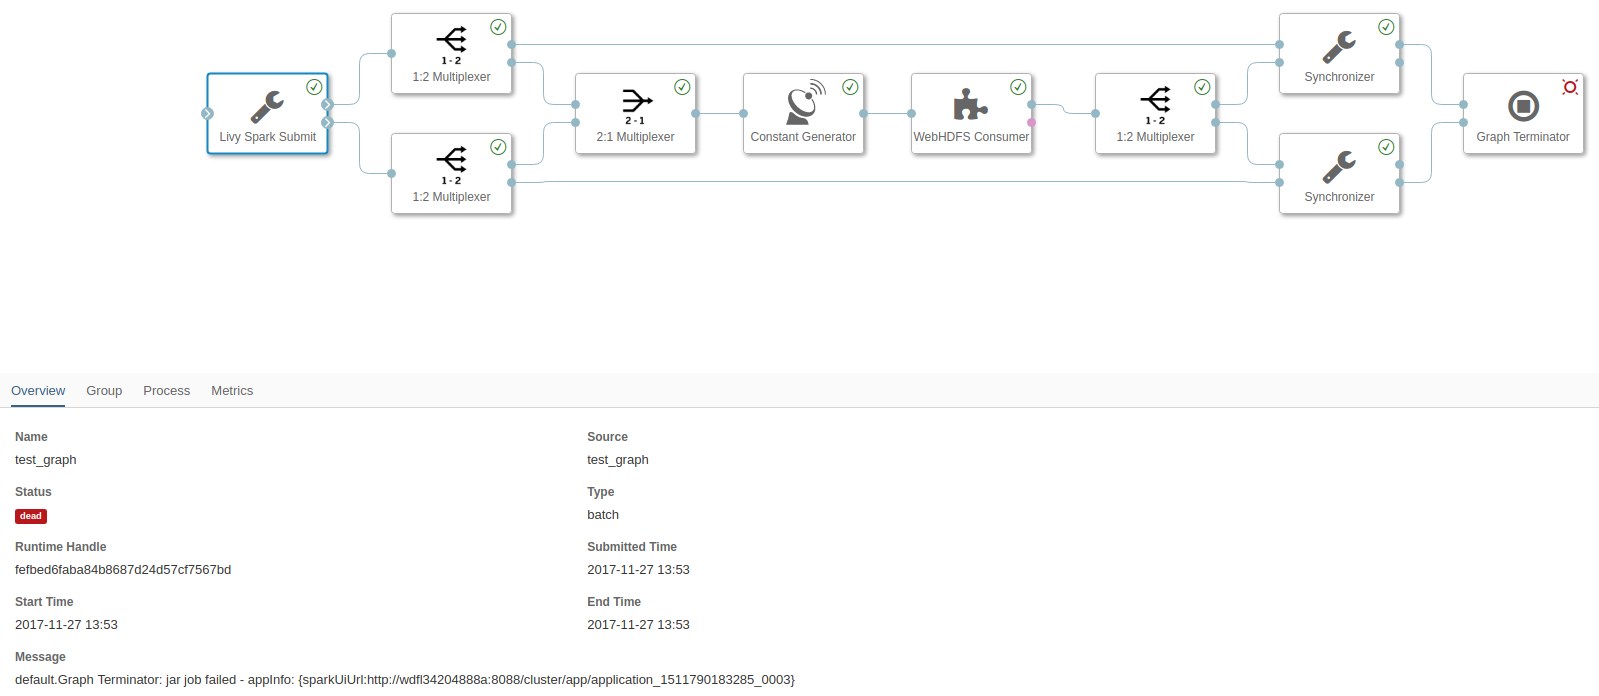
\includegraphics[width=0.88\textwidth]{pipeline_mode_failure}
		\caption{A Graph contains the Livy Operator in Pipeline Error Handling Mode}
	\end{figure}

\newpage

\section{Unit Tests \& Docker-based Integration Tests}
\setcounter{table}{0}
\setcounter{figure}{0}

As we mentioned in previous chapters, there are always bugs hidden in softwares. Those bugs produce incorrect or unexpected results, which are definitely not our wish. In order to find hidden bugs and fix them before a software is released, it has to be tested. Actually software tests could be classified into many types, but I'll focus on only 2 types that were used in my internship - unit tests and integration tests.

	\subsection{Unit Tests}
	Unit tests are typically written and run by software developers to ensure that code meets its design and behaves as intended. An unit is the smallest testable part of an application, in our case it is an individual function of the Livy operator. Ideally, each test case(unit) is independent from the others, it means a function could only cause the failure of its test case, and a test case fails only because of bugs in the function for which it is responsible. Therefore, applying unit tests has following benefits:
	
	\begin{itemize}
		\item Easy to write, a test case concentrates on just 1 function, there is need to worry about the whole architecture;
		\item Helpful for debugging, unit failures and problematic functions are bijective, developers could locate bugs precisely;
		\item Refactoring securely, a totally refactored is still reliable if it could pass the previous unit tests.
	\end{itemize}
	
	In principle, all functions should be tested in both positive and negative cases, each path of all conditional operators and loops should be covered. It is hard to write such tests for the Livy operator, because it is essentially a client-end software, many functions in it require a respond from the server, which should not appear in the unit tests, because running a real server during unit testing is way too time and resource consuming. In order to test all functions and reduce the time and resource consumption, I found a tricky solution - run a fake server that replies very simple hard-coded HTTP responds. So the efficiency problem is solved, and positive and negative cases could be easily controlled flexibly by manipulating the respond body.
		
	\subsection{Docker-based Integration Test}
	Although unit tests already provide us some methods to ensure the code quality of each components, it cannot examine the functionality of the whole software architecture. To achieve this goal, we need the integration testing, it takes components that have been unit tested as its input, groups them in larger aggregates, applies tests to those aggregates, so that defects in the interaction between components could be discovered, and the whole architecture could be tested.
	
	As we mentioned in the subsection 5.1, the largest barrier to test the Livy operator is running the server. In integration tests, strictness is more considered than efficiency, so job submissions should not be submitted to a fake server anymore, but be submitted and executed by a real "server" - actually it is a Hadoop cluster with HDFS, YARN, Spark installed, and many configurations should be done before the submitted jobs coming in.
	
	Of course it is possible to configure a virtual cluster on the computer running integration tests, however nobody does it, because the environment for testing usually conflicts with the one for development, frequently and manually changing system configurations is wasting time and very faulty, that's never the first choice. We need a tool that can deploy the above cluster and configure it automatically on any machine, and the testing environment should not influence the development. Luckily, such tool has been well-developed and it is called "Docker".
	
	Docker is a software technology provides an additional layer of abstraction and automation of operating-system-level virtualization on Windows and Linux, it allows independent "containers" to run within a single Linux instance, avoiding the overhead of starting and maintaining virtual machines.
	
	
	\begin{figure}[!h]
		\centering
		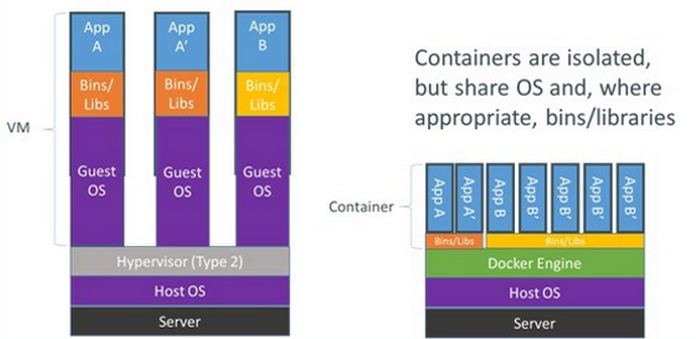
\includegraphics[width=0.63\textwidth]{docker}
		\caption{Traditional VMs vs. Docker containers\cite{what is docker}}
	\end{figure}

	All containers share the same OS base, but each of them could have its own environment variables and system configurations, so that even conflicting environments for development and testing could live together. Docker has its own script style - Dockerfile, which support automate configuring system, installing softwares, starting services, etc. Furthermore, by executing a existing Dockerfile, the identical environment could be deployed again on any machines that run docker, it's exactly the implementation of the motto "write once run anywhere".
	
	Thanks to this technology, I was able to write the integration tests without worrying about the cluster deployment and configuration conflicting.
	
	Technically, I wrote a Dockerfile that can start a container, in which a Hadoop cluster with HDFS, YARN, Spark installed is deployed, then the Dockerfile also prepares the environment variables and system configurations for the integration tests, after everything is configured, it starts all the services and uploads some libraries into the HDFS for executing jobs. Till now the preparation period is done, what we need is just start our client, submit a job to the Livy server running on the "localhost:8998"(8998 is the default port number of Livy), wait for the respond and check whether it meets the expecting result.

\newpage

\section{Conclusion}
\setcounter{table}{0}
\setcounter{figure}{0}

With the growing of big data's 3 Vs - velocity, volume and variety, it's harder and harder to process data. Improving the performance of each single server node, as known as scale up, was the first try, however it failed because of the high expense. Then distributed system was introduced, hundreds and thousands of cheap machines work together as a cluster, which has better performance, redundancy and fault tolerance than the traditional single node high performing server. In comparison, this way is called scale out. 

There are already many successful distributed data processing systems, such as Hadoop, Spark. However, they have more or less some problems that obstructs the real usage, in our case, the problem is that submitting jobs from SAP Data Hub to multiple remote Hadoop/Spark clusters is inconvenient and insecure. In order to solve this problem, a open-source project Apache Livy was introduced. A Livy server will be installed on each cluster, and a Livy client(operator) will be developed in SAP Data Hub to communicate with the remote Livy server for job submission and monitoring.

In the section 2 we have proved that Livy could fulfill all of our requirements - submitting Spark/Vora jobs to a cluster no matter it's secured by Kerberos or not. 

In the section 3 I showed how the Livy operator was designed, developed and refactored. It is true that coding is not all, but only a small part of software development, the communication between developers and customers, the plans ahead are sometimes more important, because it could save time during which we are coding in the wrong way.

In the section 4, error handling and monitoring mode is improved, errors will be returned with more detailed information for debugging. In addition, a new error handling mode "pipeline" is designed and implemented, in that mode, errors will be handled afterwards by other operators in SAP Data Hub, which provides customers great flexibility.

In the section 5, unit tests and integration tests are discussed. Each of them has characteristics, the unit testing relies on its agility and bijection to functions, so it is usually used for debugging, while the integration testing covers more codes so it is used for verifying the whole system's functionality and consistency.

Till now my work for developing the operator \textbf{Livy Spark Submit} is all explained, I learned a lot in several different perspectives - how to write code with high quality, how to discover bugs and fix them, how to communicate and cooperate with others, and so on. Being a software developer is much complexer than I thought, but I am still very interested in software engineering and want to dedicate myself to this area.

\newpage

\addcontentsline{toc}{section}{References}
\begin{thebibliography}{9}
	\bibitem{sap company information}SAP Company Information, \url{https://www.sap.com/corporate/en/company.html}
	\bibitem{sap data hub}SAP Data Hub, \url{https://www.sap.com/products/data-hub.html}
	\bibitem{data hub architecture}SAP Data Hub Architecture, \url{https://help.sap.com/viewer/e66c399612e84a83a8abe97c0eeb443a/1.2.latest/en-US/ef0654b821b345a7ac0a7468306f935c.html}
	\bibitem{vora and data hub}Installing SAP Vora and SAP Data Hub Pipeline Engine, \url{https://help.sap.com/viewer/e66c399612e84a83a8abe97c0eeb443a/1.2.latest/en-US/6d5deb33596841a3a6bd04c127a69a1d.html}
	\bibitem{vora 1.4 architecture}Vora 1.4 System Architecture, \url{https://help.sap.com/viewer/0991e2320f5940d988ed32b995d28a44/1.4/en-US/e5dfe74c499b46359bd60ca0aa9be472.html}
	\bibitem{vora 2.0 architecture}Vora 2.0 System Architecture, \url{https://help.sap.com/viewer/0991e2320f5940d988ed32b995d28a44/2.0/en-US/e5dfe74c499b46359bd60ca0aa9be472.html}
	\bibitem{vora 2.1 architecture}Vora 2.1 System Architecture, \url{https://help.sap.com/viewer/0991e2320f5940d988ed32b995d28a44/2.1/en-US/8acfad934cc347b2b52888249dfd2f20.html}
	\bibitem{what is livy}What is Livy, \url{https://livy.incubator.apache.org/}
	\bibitem{spark submit}Submitting Applications - Spark 2.2.1 Documentation, \url{https://spark.apache.org/docs/latest/submitting-applications.html}
	\bibitem{jar}JAR(file format), \url{https://en.wikipedia.org/wiki/JAR_(file_format)}
	\bibitem{hadoop}Apache Hadoop, \url{https://en.wikipedia.org/wiki/Apache_Hadoop}
	\bibitem{rest}Representational state transfer,  \url{https://en.wikipedia.org/wiki/Representational_state_transfer}
	\bibitem{curl}cURL, \url{https://en.wikipedia.org/wiki/CURL}
	\bibitem{csrf}Cross-site request forgery, \url{https://en.wikipedia.org/wiki/Cross-site_request_forgery}
	\bibitem{kerberos}Kerberos, \url{https://en.wikipedia.org/wiki/Kerberos_(protocol)}
	\bibitem{what is docker}What is Docker and why is it so darn popular?, \url{http://www.zdnet.com/article/what-is-docker-and-why-is-it-so-darn-popular/}
\end{thebibliography}

\section*{Note of Thanks}\addcontentsline{toc}{section}{Note of Thanks}
Thanks to my tutor Dr. Christian Mathis and all my colleagues, without them I couldn't adapt to the team so fast. Thanks to the knowledge I learned in TU Darmstadt, otherwise I couldn't finished this internship so successfully. Thanks to my parents and friends, their support always encourages me and make me better.

\listoffigures\addcontentsline{toc}{section}{\listfigurename}
  
\end{document}
